\section{What the negotiated positions become}
\label{sec:economy}

\subsection{Development has a financing path and an exposure history}

The agents' concerns about building funds correspond to a real transition between completing a group and raising its rent schedule. All sixty-three trade-completed groups reach a management window. Forty-three receive construction in that first window: sixteen of seventeen for Sol, seventeen of eighteen for Gemini, seven of fifteen for Opus, and three of thirteen for Grok. The remaining twenty divide into nine without an offered build on the target group, four defaults, four received-call disagreements, and three other valid ends. Completion counts by themselves conceal these different opportunities and outcomes.

Eight of the nine groups without a build option contain a mortgage. Two owners have enough cash at window entry to cover the implemented redemption price and one house; five more have sufficient budgets if currently offered outside-group mortgages are included. These are static budgets, not new executed financing routes. Grok's four notes explicitly defer redemption or construction for liquidity. Such a deferral can preserve cash while sacrificing immediate rent, and mortgaging other collateral may disable a different group. The record does not supply a common objective that ranks those choices.

Response handling contributes a separate path. The historical checks preserve all sixty-one defaulted Opus construction purchase multisets after legally splitting and ordering the requested purchases. Their submitted encodings remain invalid. Sixty chains contain refusal followed by invalid recovery, while G2 d129 contains invalid construction followed by refusal. Exhausting the response budget ends management. This is evidence about requested allocations and execution, not evidence that those allocations were good investments or that a corrected interface would change a winner. Details remain in the appendix rather than becoming a defect taxonomy in the main argument.

\begin{table}[t]
\centering\small
\begin{tabular}{@{}lrr@{}}\toprule
Trade-completed episode measure & Built in first window & Other\\\midrule
Episodes & 43 & 20\\
Median completion turn & 66 & 69.5\\
Median ownership duration, turns & 62 & 63.5\\
Median opponent movement events & 42 & 47\\
Total opponent movement events & 2,518 & 1,029\\
Group landings during ownership & 150 & 63\\
Paid rent during ownership & \$53,810 & \$3,568\\\bottomrule
\end{tabular}
\caption{Fresh arithmetic over preserved episode boundaries and original movement events. Rent sums match the inherited episode ledger. Landings include mortgaged and nonpaying deeds. Opponent movements count realized exposure; they are affected by the course of play.}
\label{tab:exposure}
\end{table}

The first-window groups collect 93.8\% of paid rent after trade completion, a magnitude previously easy to confuse with a return to early development. Table~\ref{tab:exposure} now shows the associated timing and exposure. Median acquisition dates and ownership durations are similar, and the non-first-window group actually has the larger median movement exposure. At the aggregate level, the first-window groups account for 71.0\% of opponent movements and 70.4\% of group landings. Their 93.8\% rent share is therefore not solely a consequence of having nearly all the observed landings.

This decomposition makes the economic history more informative without identifying a treatment effect. Paid rent per recorded group landing is about \$359 versus \$57; it combines the rent schedule, mortgages, payer resources, acquisition route, and later development. Eleven of the twenty comparison episodes build later. A fatal rent demand can produce an estate instead of a paid-rent event. Movement is endogenous to survival and decisions, and multiple groups can share the same opponent move in their exposure totals. Figure~\ref{fig:exposure} retains every episode so that a long-lived unproductive acquisition is not confused with an acquisition just before termination.

\begin{figure}[p]
\centering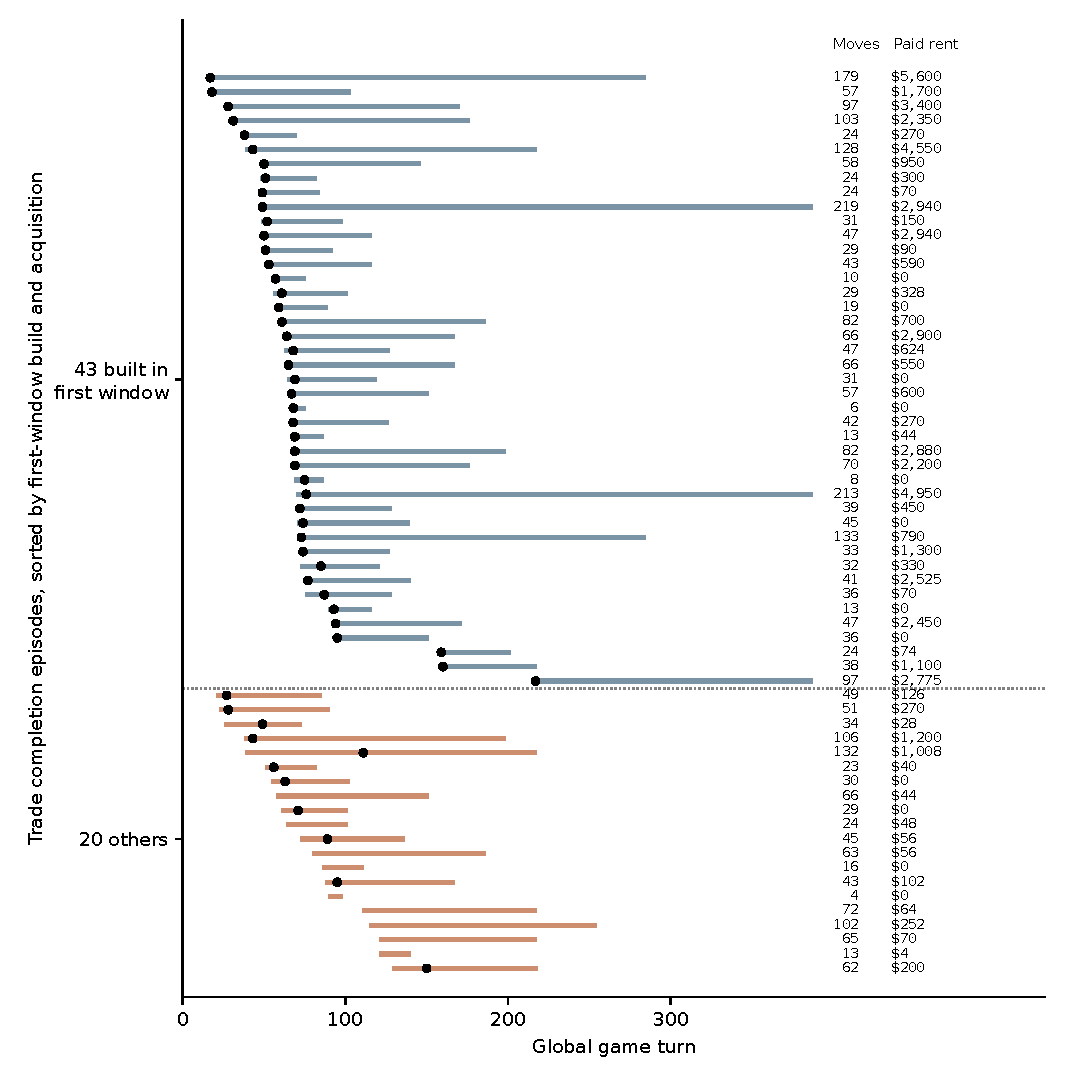
\includegraphics[width=.95\linewidth,height=.77\textheight,keepaspectratio]{exposure.pdf}
\caption{Ownership intervals for all sixty-three trade-completed groups. Blue rows receive construction in the first management window; brown rows do not. Black points show first construction where observed. Rows are sorted within each class by acquisition turn and game; the paired columns give opponent moves and paid rent. Horizontal coordinates are global turns within each episode's own game. Empty black-point histories remain visible. Exact row identities and measures are preserved in \texttt{data/development\_exposure.json}.}
\label{fig:exposure}
\end{figure}

Planning appears at this same boundary between an expressed target and a later opportunity. Sol's G9 turn-29 note sets a target of three houses on each dark-blue deed; recorded financing and construction reach it at turn 60. Conversely, Grok's G16 named-property purchase plan encounters an affordable Virginia menu, and its note still favors purchase, but the received call starts an auction. A prior 240-decision textual sample contains many contingent statements and few later matched opportunities. We retain the concrete positive and conflicting trajectories rather than turning that selected sample into a planning rate. Neither target realization nor recurrence alone identifies the contribution of private-note memory.

\subsection{Successful financing changes the debt denominator}

The full debt-menu population contains 188 episodes. In 128, the final action emits payment of the recorded amount. The other sixty match the elimination ledger. Its inherited classifications identify three legal payment routes, fifty-six debts beyond the generous own-asset bound, and one menu-level hotel lock. Table~\ref{tab:debts} puts successful and unsuccessful outcomes together. Among the 131 demonstrably payable episodes, three end in elimination, or 2.3\%. This is an exact corpus description using observed payments and existing witnesses. It is not an estimate of general financial competence, and it does not include ordinary bills paid immediately without reaching a debt menu.

\begin{table}[t]
\centering\small
\begin{tabular}{@{}lrrrr@{}}\toprule
Configuration & Paid & Payable elimination & Bound below debt & Menu lock\\\midrule
Sol & 30 & 1 & 11 & 0\\
Gemini & 37 & 1 & 12 & 0\\
Opus & 41 & 0 & 16 & 1\\
Grok & 20 & 1 & 17 & 0\\\midrule
All & 128 & 3 & 56 & 1\\\bottomrule
\end{tabular}
\caption{All episodes reaching liquidation. Paid endpoints are freshly matched to emitted payment events; elimination feasibility uses inherited engine witnesses or bounds. Counts condition on different histories and do not rank configurations.}
\label{tab:debts}
\end{table}

Sol's G20 payment illustrates the scale of successful finance. Starting with \$49, it raises \$700 in building salvage and \$665 through mortgages, pays \$1,400, and retains \$14. Gemini's G16 note instead correctly concludes that \$288 cash, \$375 salvage, and \$730 mortgages total only \$1,393 against a \$2,000 debt. These are different kinds of competence evidence: an executed multistep payment and a correct recognition of insolvency. The population denominator prevents a few payable eliminations from standing for every encounter with financial distress.

\Incident{g12}{A payment route is recognized but a different action executes}

Grok owes \$250 and has \$43. Its pinks hold two, two, and three houses. Assistant content requests a two-house Virginia sale, while its private note concludes:
\TranscriptQuote{g12_d249_private_final}
The received tool call instead declares bankruptcy:
\TranscriptQuote{g12_d249_public_bankruptcy}
The engine eliminates Grok and transfers the estate to Opus. The inherited five-sale sequence pays the debt and leaves \$43. The two-house sale named in content is legal but insufficient, reaching only \$143. Grok's full private field moves from an initial impossibility claim to a sufficient five-sale calculation, although it miscounts the houses remaining. The recorded public field supports bankruptcy, but no later recipient request carries it. Recognition, a partial proposed action, and the applied declaration are therefore distinct observations. Calling this simply a failure to reason about liquidation would discard relevant evidence; calling it a deliberate surrender would also exceed the record.
\Source{G12 d249, standard attempt 0; quote spans freshly checked, five-sale feasibility inherited from the historical witness suite.}

The menu lock has a different interpretation. At G7 d339, Opus owes \$750, has \$390, and can mortgage Oriental for \$50. Its pinks contain four houses, four houses, and a hotel, but the bank has no houses. The menu offers no sale because the highest-built deed is a hotel and downgrade needs four bank houses. The retained mortgage-only continuation reaches \$440 despite \$1,310 nominal resources. This case concerns finance accessible through the actual menu. It should neither be counted as an irrational refusal to use an offered sale nor silently removed to make the experiment cleaner.

\subsection{Creditor positions precede the estate}

Before the final elimination, estates transfer 227 deeds, 202 to eventual winners. The first creditor wins eighteen games. Those figures motivate asking what position the creditor already held. Figure~\ref{fig:estate} shows ranks immediately before the first bankruptcy action. First creditors lead or tie in prior paid rent in fifteen games and in building house-equivalents in twelve, but lead or tie in cash in only eight. They are not uniformly the cash-richest or most asset-rich players. They often already hold a rent-producing position before the estate arrives.

\begin{figure}[t]
\centering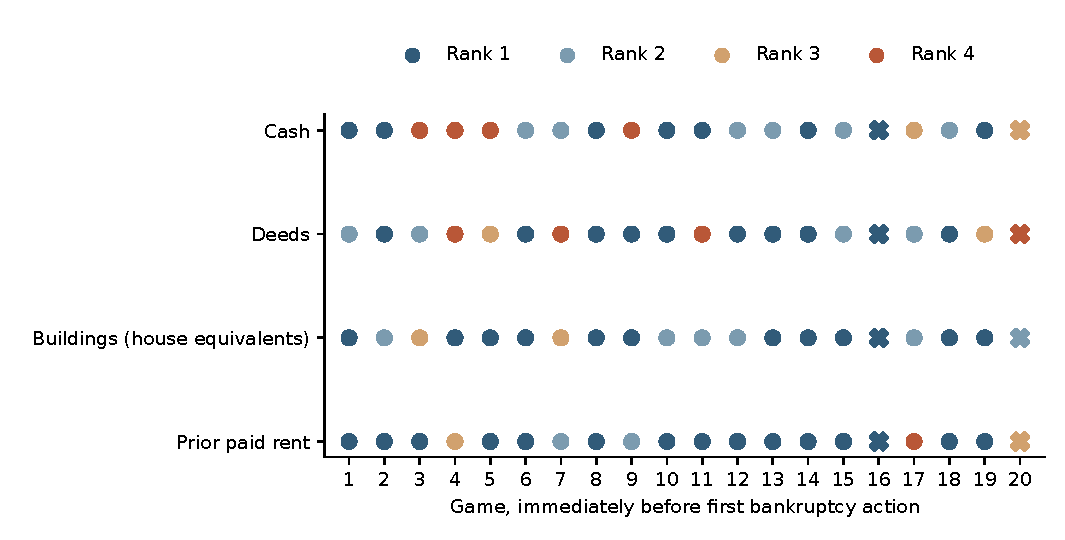
\includegraphics[width=\linewidth]{pre_estate.pdf}
\caption{First creditor's pre-estate rank among all four players. Rank one includes ties. Crosses mark the two games whose first creditor does not eventually win. Prior paid rent is cumulative receipts before the elimination; building equivalents count a hotel as five construction levels. This case-level display describes prior position without fitting a winner predictor.}
\label{fig:estate}
\end{figure}

The incoming assets still matter to the continuing game. Nonterminal estates complete fifty-two groups, forty-five for eventual winners, and transfer buildings intact under this ruleset. Yet only fourteen of those fifty-two groups receive any subsequent rent, compared with fifty-one of sixty-three trade-completed groups. Late acquisition and existing dominance restrict further opportunities. Counting terminal estate completions as productive achievements would be especially misleading because sixty-nine occur at the final elimination and have no later management window. These histories make prospective creditor identity a plausible bargaining concern while leaving its independent contribution to victory unmeasured.

\Incident{g13}{A seller uses creditor succession to frame a cash demand}

Grok stands on Atlantic with \$35, nine squares before Sol's Short Line, where a landing costs \$200. It offers mortgaged Pennsylvania to Opus for \$200 and says Sol would otherwise inherit its yellows. Opus counters \$130. Grok replies:
\TranscriptQuote{g13-seller-counter}
Ventnor is unmortgaged and supplies \$130 if mortgaged. Grok's returned provider explanation explicitly identifies the omission:
\TranscriptQuote{g13-omission-explanation}
Opus pays \$200 plus \$16 transfer interest. Its returned explanation repeats the estate concern, but does not endorse the claimed financing limit. Under the retained conditional branch, \$130 purchase cash, Grok's \$35, and a \$130 Ventnor mortgage total \$295, enough for the threatened rent. The original opening also gives an inaccurate first-roll probability. Its 5/36 claim does not equal the 4/36 first-roll sum for nine squares; either figure alone omits additional movement through doubles and cards.

Grok avoids Short Line on its next roll, later pays \$200 on B\&O, and eventually fails on Short Line at turn 150. Seven turns after the trade, Opus buys North Carolina for \$650 and completes green with the acquired Pennsylvania. The account thus contains a concrete omitted alternative, a settled transaction, and an echoed concern about a third-party creditor. It does not identify the omission as the cause of the additional \$70 or quantify survival purchased by the deal.
\Source{G13 d250--253, d307 and d311; green auction event 1911. Grok uses standard responses; Opus uses recovery. Conditional finance is inherited, not executed anew.}

\Incident{g18}{A repeated assurance is withdrawn after financial deterioration}

Opus repeatedly offers \$250 for Sol's mortgaged Pacific, which would complete its greens. After collecting \$750 from Sol it reiterates:
\TranscriptQuote{g18-assurance}
A second \$750 payment forces Sol to sell buildings and mortgage remaining red deeds, leaving \$49. Sol invokes the price, and Opus withdraws:
\TranscriptQuote{g18-invocation}
\TranscriptQuote{g18-withdrawal}
Opus's returned explanation says paying would briefly prolong a nearly bankrupt rival and that its own greens still need redemption and construction. It subsequently redeems Pennsylvania and North Carolina, then offers \$150 and \$225 for Pacific. Sol asks more, and no deal settles. Opus eventually acquires Sol's estate and wins. Portfolio changes between withdrawal and later bids alter the marginal cost of completing green, so resumed bidding does not refute a state-dependent valuation. The earlier assurance is received but unenforced; no costly reliance or dishonest original intention is established. The strategically relevant change is the buyer's stated value of extending a rival's life as the estate becomes nearer.
\Source{G18 d421--461. Quotes come from applied public fields under Opus recovery. The withdrawal explanation is provider-returned text, not an authored private-memory note.}
